%%%%%%%%%%%%%%%%%%%%%%%%%%%%%%%%%%%%%%%%%
% Classicthesis Typographic Thesis
% LaTeX Template
% Version 1.1 (4/8/12)
%
% This template has been downloaded from:
% http://www.LaTeXTemplates.com
%
% Original author:
% André Miede (http://www.miede.de)
%
% License:
% CC BY-NC-SA 3.0 (http://creativecommons.org/licenses/by-nc-sa/3.0/)
%
% General Tips:
% 1) Make sure to edit the classicthesis-config.file
% 2) New enumeration (A., B., C., etc in small caps): %\begin{aenumerate} \end{aenumerate}
% 3) For margin notes: \marginpar or \graffito{}
% 4) Do not use bold fonts in this style, it is designed around them
% 5) Use tables as in the examples
% 6) See classicthesis-preamble.sty for useful commands
%
%%%%%%%%%%%%%%%%%%%%%%%%%%%%%%%%%%%%%%%%%

%----------------------------------------------------------------------
%	PACKAGES AND OTHER DOCUMENT CONFIGURATIONS
%---------------------------------------------------------------------

\documentclass[
		oneside,openright,titlepage,numbers=noenddot,headinclude,%1headlines,
                footinclude=true,cleardoublepage=empty,
                BCOR=5mm,paper=a4,fontsize=12pt, % Binding correction, paper type and font size
                american, % Languages
                ]{scrreprt} 
                
% Includes the file which contains all the document configurations and packages - make sure to edit this file
%%%%%%%%%%%%%%%%%%%%%%%%%%%%%%%%%%%%%%%%%
% Thesis Configuration File
%
% The main lines to change in this file are in the DOCUMENT VARIABLES
% section, the rest of the file is for advanced configuration.
%
%%%%%%%%%%%%%%%%%%%%%%%%%%%%%%%%%%%%%%%%%

%----------------------------------------------------------------------------------------
%	DOCUMENT VARIABLES
%	Fill in the lines below to enter your information into the thesis template
%	Each of the commands can be cited anywhere in the thesis
%----------------------------------------------------------------------------------------

% Remove drafting to get rid of the '[ Date - classicthesis version 4.0 ]' text at the bottom of every page
\PassOptionsToPackage{eulerchapternumbers,subfig,beramono,eulermath,subfig,drafting}{classicthesis}
% Available options: drafting parts nochapters linedheaders eulerchapternumbers beramono eulermath pdfspacing minionprospacing tocaligned dottedtoc manychapters listings floatperchapter subfig
% Adding 'dottedtoc' will make page numbers in the table of contents flushed right with dots leading to them

\newcommand{\myTitle}{A Classic Thesis Style\xspace}
\newcommand{\mySubtitle}{An Homage to The Elements of Typographic Style\xspace}
\newcommand{\myDegree}{Doktor-Ingenieur (Dr.-Ing.)\xspace}
\newcommand{\myName}{Andr\'e Miede\xspace}
\newcommand{\myProf}{Put name here\xspace}
\newcommand{\myOtherProf}{Put name here\xspace}
\newcommand{\mySupervisor}{Put name here\xspace}
\newcommand{\myFaculty}{Put data here\xspace}
\newcommand{\myDepartment}{Put data here\xspace}
\newcommand{\myUni}{Put data here\xspace}
\newcommand{\myLocation}{Darmstadt\xspace}
\newcommand{\myTime}{December 2011\xspace}
\newcommand{\myVersion}{version 4.0\xspace}

%----------------------------------------------------------------------------------------
%	USEFUL COMMANDS
%----------------------------------------------------------------------------------------

\newcommand{\ie}{i.\,e.}
\newcommand{\Ie}{I.\,e.}
\newcommand{\eg}{e.\,g.}
\newcommand{\Eg}{E.\,g.} 

\newcounter{dummy} % Necessary for correct hyperlinks (to index, bib, etc.)
\providecommand{\mLyX}{L\kern-.1667em\lower.25em\hbox{Y}\kern-.125emX\@}

%----------------------------------------------------------------------------------------
%	PACKAGES
%----------------------------------------------------------------------------------------
% Added by Lisa

% font select changes
\usepackage{everysel}
% linguistic examples
% http://en.wikibooks.org/wiki/LaTeX/Linguistics#Enumerated_examples
\usepackage{linguex}
%\usepackage{gb4e}
%----------------------------------------------------------------------------------------

\usepackage{lipsum} % Used for inserting dummy 'Lorem ipsum' text into the template

%------------------------------------------------
 
\PassOptionsToPackage{latin9}{inputenc} % latin9 (ISO-8859-9) = latin1+"Euro sign"
\usepackage{inputenc}
 
 %------------------------------------------------

%\PassOptionsToPackage{ngerman,american}{babel}  % Change this to your language(s)
% Spanish languages need extra options in order to work with this template
%\PassOptionsToPackage{spanish,es-lcroman}{babel}
\usepackage{babel}

%------------------------------------------------			


%\usepackage[nosectionbib]{apacite}

\usepackage{apacite}
\usepackage{makerobust}
\DeclareRobustCommand{\citep}[2][]{\cite[#1]{#2}}
\DeclareRobustCommand{\citealp}[2][]{\citeNP[#1]{#2}}
\DeclareRobustCommand{\citet}[2][]{\citeA[#1]{#2}}
\MakeRobustCommand{\citeauthor}
\MakeRobustCommand{\citeauthor}

\PassOptionsToPackage{round}{natbib}
\usepackage{natbib}

 %------------------------------------------------

\PassOptionsToPackage{fleqn}{amsmath} % Math environments and more by the AMS 
 \usepackage{amsmath}
 
 %------------------------------------------------

\PassOptionsToPackage{T1}{fontenc} % T2A for cyrillics
\usepackage{fontenc}

%------------------------------------------------

\usepackage{xspace} % To get the spacing after macros right

%------------------------------------------------

\usepackage{mparhack} % To get marginpar right

%------------------------------------------------

\usepackage{fixltx2e} % Fixes some LaTeX stuff 

%------------------------------------------------

\PassOptionsToPackage{smaller}{acronym} % Include printonlyused in the first bracket to only show acronyms used in the text
\usepackage{acronym} % nice macros for handling all acronyms in the thesis

%------------------------------------------------

%\renewcommand*{\acsfont}[1]{\textssc{#1}} % For MinionPro
\renewcommand{\bflabel}[1]{{#1}\hfill} % Fix the list of acronyms

%------------------------------------------------

\PassOptionsToPackage{pdftex}{graphicx}
\usepackage{graphicx} 

%----------------------------------------------------------------------------------------
%	FLOATS: TABLES, FIGURES AND CAPTIONS SETUP
%----------------------------------------------------------------------------------------

\usepackage{tabularx} % Better tables
\setlength{\extrarowheight}{3pt} % Increase table row height
\newcommand{\tableheadline}[1]{\multicolumn{1}{c}{\spacedlowsmallcaps{#1}}}
\newcommand{\myfloatalign}{\centering} % To be used with each float for alignment
\usepackage{caption}
\captionsetup{format=hang,font=small}
\usepackage{subfig}  

%----------------------------------------------------------------------------------------
%	CODE LISTINGS SETUP
%----------------------------------------------------------------------------------------

\usepackage{listings} 
%\lstset{emph={trueIndex,root},emphstyle=\color{BlueViolet}}%\underbar} % for special keywords
\lstset{language=[LaTeX]Tex, % Specify the language for listings here
keywordstyle=\color{RoyalBlue}, % Add \bfseries for bold
basicstyle=\small\ttfamily, % Makes listings a smaller font size and a different font
%identifierstyle=\color{NavyBlue}, % Color of text inside brackets
commentstyle=\color{Green}\ttfamily, % Color of comments
stringstyle=\rmfamily, % Font type to use for strings
numbers=left, % Change left to none to remove line numbers
numberstyle=\scriptsize, % Font size of the line numbers
stepnumber=5, % Increment of line numbers
numbersep=8pt, % Distance of line numbers from code listing
showstringspaces=false, % Sets whether spaces in strings should appear underlined
breaklines=true, % Force the code to stay in the confines of the listing box
%frameround=ftff, % Uncomment for rounded frame
frame=single, % Frame border - none/leftline/topline/bottomline/lines/single/shadowbox/L
belowcaptionskip=.75\baselineskip % Space after the "Listing #: Desciption" text and the listing box
}

%----------------------------------------------------------------------------------------
%	HYPERREFERENCES
%----------------------------------------------------------------------------------------

\PassOptionsToPackage{pdftex,hyperfootnotes=false,pdfpagelabels}{hyperref}
\usepackage{hyperref}  % backref linktocpage pagebackref
\pdfcompresslevel=9
\pdfadjustspacing=1

\hypersetup{
% Uncomment the line below to remove all links (to references, figures, tables, etc)
%draft, 
colorlinks=true, linktocpage=true, pdfstartpage=3, pdfstartview=FitV,
% Uncomment the line below if you want to have black links (e.g. for printing black and white)
%colorlinks=false, linktocpage=false, pdfborder={0 0 0}, pdfstartpage=3, pdfstartview=FitV, 
breaklinks=true, pdfpagemode=UseNone, pageanchor=true, pdfpagemode=UseOutlines,
plainpages=false, bookmarksnumbered, bookmarksopen=true, bookmarksopenlevel=1,
hypertexnames=true, pdfhighlight=/O, urlcolor=webbrown, linkcolor=RoyalBlue, citecolor=webgreen,
%------------------------------------------------
% PDF file meta-information
pdftitle={\myTitle},
pdfauthor={\textcopyright\ \myName, \myUni, \myFaculty},
pdfsubject={},
pdfkeywords={},
pdfcreator={pdfLaTeX},
pdfproducer={LaTeX with hyperref and classicthesis}
%------------------------------------------------
}   

%----------------------------------------------------------------------------------------
%	BACKREFERENCES
%----------------------------------------------------------------------------------------

\usepackage{ifthen} % Allows the user of the \ifthenelse command
\newboolean{enable-backrefs} % Variable to enable backrefs in the bibliography
\setboolean{enable-backrefs}{false} % Variable value: true or false

\newcommand{\backrefnotcitedstring}{\relax} % (Not cited.)
\newcommand{\backrefcitedsinglestring}[1]{(Cited on page~#1.)}
\newcommand{\backrefcitedmultistring}[1]{(Cited on pages~#1.)}
\ifthenelse{\boolean{enable-backrefs}} % If backrefs were enabled
{
\PassOptionsToPackage{hyperpageref}{backref}
\usepackage{backref} % to be loaded after hyperref package 
\renewcommand{\backreftwosep}{ and~} % separate 2 pages
\renewcommand{\backreflastsep}{, and~} % separate last of longer list
\renewcommand*{\backref}[1]{}  % disable standard
\renewcommand*{\backrefalt}[4]{% detailed backref
\ifcase #1 
\backrefnotcitedstring
\or
\backrefcitedsinglestring{#2}
\else
\backrefcitedmultistring{#2}
\fi}
}{\relax} 

%----------------------------------------------------------------------------------------
%	AUTOREFERENCES SETUP
%	Redefines how references in text are prefaced for different 
%	languages (e.g. "Section 1.2" or "section 1.2")
%----------------------------------------------------------------------------------------

\makeatletter
\@ifpackageloaded{babel}
{
\addto\extrasamerican{
\renewcommand*{\figureautorefname}{Figure}
\renewcommand*{\tableautorefname}{Table}
\renewcommand*{\partautorefname}{Part}
\renewcommand*{\chapterautorefname}{Chapter}
\renewcommand*{\sectionautorefname}{Section}
\renewcommand*{\subsectionautorefname}{Section}
\renewcommand*{\subsubsectionautorefname}{Section}
}
\addto\extrasngerman{
\renewcommand*{\paragraphautorefname}{Absatz}
\renewcommand*{\subparagraphautorefname}{Unterabsatz}
\renewcommand*{\footnoteautorefname}{Fu\"snote}
\renewcommand*{\FancyVerbLineautorefname}{Zeile}
\renewcommand*{\theoremautorefname}{Theorem}
\renewcommand*{\appendixautorefname}{Anhang}
\renewcommand*{\equationautorefname}{Gleichung}
\renewcommand*{\itemautorefname}{Punkt}
}
\providecommand{\subfigureautorefname}{\figureautorefname} % Fix to getting autorefs for subfigures right
}{\relax}
\makeatother

%----------------------------------------------------------------------------------------

\usepackage{classicthesis} 

%----------------------------------------------------------------------------------------
%	CHANGING TEXT AREA 
%----------------------------------------------------------------------------------------

%\linespread{1.05} % a bit more for Palatino
%\areaset[current]{312pt}{761pt} % 686 (factor 2.2) + 33 head + 42 head \the\footskip
%\setlength{\marginparwidth}{7em}%
%\setlength{\marginparsep}{2em}%

%----------------------------------------------------------------------------------------
%	USING DIFFERENT FONTS
%----------------------------------------------------------------------------------------

%\usepackage[oldstylenums]{kpfonts} % oldstyle notextcomp
%\usepackage[osf]{libertine}
%\usepackage{hfoldsty} % Computer Modern with osf
%\usepackage[light,condensed,math]{iwona}
%\renewcommand{\sfdefault}{iwona}
%\usepackage{lmodern} % <-- no osf support :-(
%\usepackage[urw-garamond]{mathdesign} <-- no osf support :-(

\begin{document}

% Switch fonts easily
\EverySelectfont{%
\fontdimen2\font=0.4em% interword space
\fontdimen3\font=0.2em% interword stretch
\fontdimen4\font=0.1em% interword shrink
\fontdimen7\font=0.1em% extra space
\hyphenchar\font=`\-% to allow hyphenation
}
\newenvironment{exfont}{\fontfamily{pcr}\selectfont}{\par}
%\def\hyph{-\penalty0\hskip0pt\relax}
\newenvironment{sloppier}
{\sloppy}

\frenchspacing % Reduces space after periods to make text more compact

\raggedbottom % Makes all pages the height of the text on that page


\selectlanguage{american} % Select your default language - e.g. american or ngerman

%\renewcommand*{\bibname}{new name} % Uncomment to change the name of the bibliography
%\setbibpreamble{} % Uncomment to include a preamble to the bibliography - some text before the reference list starts

\pagenumbering{roman} % Roman page numbering prior to the start of the thesis content (i, ii, iii, etc)

%\pagestyle{plain} % Suppress headers for the pre-content pages
% page number on bottom right
\pagestyle{scrheadings}
\clearscrplain
\rofoot[\pagemark]{\pagemark}


%----------------------------------------------------------------------------------------
%	PRE-CONTENT THESIS PAGES
%----------------------------------------------------------------------------------------

\pagestyle{scrheadings} % Show chapter titles as headings
\clearscrplain

\pagenumbering{arabic} % Arabic page numbering for thesis content (1, 2, 3, etc)

\cleardoublepage % Avoids problems with pdfbookmark

%----------------------------------------------------------------------------------------
%	THESIS CONTENT - CHAPTERS
%----------------------------------------------------------------------------------------
 
\chapter{Introduction}
\label{introduction}

 \begin{quote} 

All forms of communication entail design, as the intent of communication is to be understood by others or by one's self at another time. Communication design, then, is inherently social, because to be understood by another or by self at another time entails fashioning communications to fit the presumed mental states of others or of one's self at another time.  \citep[p. 6]{Tversky:2010ww} 
 \end{quote} 

\section{Mis-Communication in Interaction Design}
\label{mis-communicationininteractiondesign}

Good interaction design takes into account user cognitive processes and limitations. The current state of practice is richly informed by an understanding of perception, attention, memory, categorization, learning, decision-making, and comprehension. Though designers spend considerable effort toward producing user interfaces and interactions that communicate effectively, the tools that they use are flexible can easily bend to either inadvertently or intentionally cause users to make incorrect inferences about the situation at hand. Because graphical users interfaces (GUIs) share properties with other forms of communication such as language, gesture, diagrams and action and are inherently interactional, \emph{I argue that they are also subject to the same context-dependent aspects of meaning that arise with the use of language}. 

In traditional GUI-based interaction, user interactions are designed. When a user interacts with a website, that interaction is structured according to that site designer's plan. Ideally, information has been organized with user expectation in mind. The designer has considered the sorts of tasks users intend to perform. Sometimes, navigation is guided. Sometimes not, but designers leave behind contextual cues and guideposts to aid users in their task. Nearly always, the designer intends to create an interaction that is as free from confusion as possible. Or does he?

There are situations where confusion may be desirable. Or, if not confusion, then understanding of how to design an interaction in such a way to appear fair and equitable, but in actuality, influence a user to act in very predictable ways. Psychologist Amos Tversky, and later Tversky and Kahneman, produced ground-breaking work in behavioral economics showing how non-rational behavioral could be identified and predicted. For example, Kahneman and Tversky  \citeyearpar{Tversky:1981vc}  showed that predictable, dramatic shifts in preference could be generated simply by changing the ways options are framed: in early framing experiments, subjects showed a preference toward risk aversion when lotteries were framed as gains, and risk seeking when lotteries were framed as losses. As noted by  \citet*{Thaler:2010uy} , designers have the potential for great control over user decision-making by manipulating behavior using psychological tools described by theoretical psychologists and behavioral economists.

Language operates using the same principles and processes as other cognitive functions. It is not surprising to learn that language can be used to manipulate hearer understanding. For example,
 
\lb{example1}{\begin{exfont}The Sheriff caught Robin red-handed. He is now serving time in prison.\end{exfont}}

Sentence 1 above appears to convey the following facts that weren't explicitly stated:

\lbu{im1}{example1}{\(a\)}{\begin{exfont}\emph{It is Robin who is serving time in prison.}\end{exfont}}
\lbu{im2}{example1}{\(b\)}{\begin{exfont}\emph{Robin is serving time in prison as a result of being caught red-handed by the Sheriff.}\end{exfont}}

These un-stated propositions (1a) and (1b) are known as \emph{implicatures}, a well-known pragmatic phenomenon in language understanding. In fact, depending on situational context, either of these implicatures may not be true\footnote{Imagine that `the Sheriff' is `the Sheriff of Nottingham', and `Robin' is `Robin Hood'. The Sheriff caught Robin Hood returning illegal taxes back to the citizenry. Later, the Sheriff was jailed for fraud. This is a somewhat implausible interpretation because we expect the second sentence in the example to have a causal relation to the first. 

But imagine now that these two sentences are captions in a humorous movie. Visual scenes serve as a contextual backdrop against implicatures in the text. In this context, the propositions raised by implicature are false.}. Implicatures operate under principles such that we may presume their truth even if un-stated. But if the truth value of either implicature turns out to be false, this does not mean that (1) is false.

Of course, it is very easy to see how language can be used to manipulate understanding, but is it possible for GUIs to communicate in the same sort of way? I believe so. The manipulation of discourse understanding is a powerful tool with subtle but important influence. This dissertation will argue that GUI-based mis-communications may be brought about by faulty pragmatic inferences. This class of mis-communications in user interaction design has not yet been described nor explained in academic literature; this dissertation addresses this gap.

\section{Pragmatics in Discourse Understanding}
\label{pragmaticsindiscourseunderstanding}

Discourse is generally said to encompass language use beyond the bounds of a sentence or proposition. It is often associated with the study of pragmatics. As Stalnaker  \citeyearpar[p. 34]{Stalnaker:1999vl}  puts it, ``Syntax studies sentence. Semantics studies propositions. Pragmatics is the study of linguistic acts and the contexts in which they are performed.'' Pragmatics attempt to account for meaning of messages where actual meaning is underdetermined from what is said. Phenomena of study include implicature (as exemplified above), presupposition, speech acts, and deixis  \citep{Huang:2007ww}.  

Pragmatics is fundamentally concerned with reasoning processes that go beyond conventional meaning to interpretation in situational and belief contexts. It is founded on the notion of language as actions with communicative goals  \citep{Grice:1975vz,Levinson:2000ud,Clark:1996tm} . According to an inferential model, ``hearers'' infer a ``speaker's'' meaning on the basis of evidence provided. In a linguistic tradition of discourse analysis, lexical, grammatical, and structural properties of language serve as a source for inference. 

Discourse is also studied by sociologists, anthropologists, and sociolinguists. In this vein, discourse is bound to socio-cultural knowledge and is governed by social norms which are shared, culturally specific aspects of interpretation  \citep{Gumperz:1982tc,Hymes:1974wr}.  Even so, discursive communication is seen as structured both in terms of conversational events such as statement and response to learned, ritualistic schemas such as making a phone reservation  \citep{Goffman:1981tm}.  In this tradition, conversational inferences are also context-bound but conceived more generally as preferences, maxims, or tendencies.

\section{Graphical Communication}
\label{graphicalcommunication}

 \graffito{Should this section be edited for simpler language and fewer references?} 

There is reason to think that messages produced by graphical user interfaces may be interpreted under the same inferential model of communication as language. Stenning, Lascarides, and Calder  \citeyearpar[p. 476]{Stenning:2006wu}  define graphics as ``planar displays of information that use the distribution of shapes, patterns, and annotations and the relation between them to convey information.'' Barbara Tversky  \citeyearpar{Tversky:2004wj,Tversky:2010ww}  summarizes a body of psychological experimentation demonstrating parallels between graphics, gesture, and language. Shared cognitive principles allow for mapping between visual and verbal modes in a number of domains. For example, Oberlander  \citeyearpar{Oberlander:1995vv}  argues for graphical implicature in the use of graphical notations for computer-assisted design in electronics. Such meanings of schematic visual forms (glyphs and other devices) convey and constrain meaning  \citep{Tversky:2010ww}.  Glyphs also combine into complex diagrams using domain-specific syntax rules  \citep*{Tversky:1999ta}.  Tversky  \citeyearpar{Tversky:2010ww}  notes that glyphs may be used to abstractly represent a variety of concepts such as objects, collections, relations, and processes. Such representations participate in cognitive processes such as ``inference, analogy, generalization, transfer, and insight.''  \citep[p. 2]{Tversky:2010ww} 

Though graphics and language differ in expressiveness and information packaging, they can both be studied using pragmatic theory  \citep*{Stenning:2002vd,Stenning:1995ka}.  Johnson-Laird  \citeyearpar{JohnsonLaird:1989uj}  describes the machinery by which linguistic representations (logical syllogisms expressed graphically) can be used to construct and update a mental model.\footnote{Mental models are equivalent to discourse models  \citep*{JohnsonLaird:1980uf}.  However, the term ``discourse model'' is preferred here as it is has been more widely adopted by researchers in the academic traditions discussed.} A discourse model is an important construct for inferencing. As discourse proceeds, the discourse model is revised to accommodate new beliefs, but is also subject to revision when conflicting information arises. The notion of a discourse model has been crucial to theory in linguistics that accommodates a wide range of phenomena to include anaphora, tense, and presupposition. But discourse models have also been applied to graphical reasoning where such representations are posited as a means to achieve efficiency in cognitive processing given constraints in working memory  \citep*{Stenning:1995ka}. 

\section{Confusion in Online Behavioral Advertising}
\label{confusioninonlinebehavioraladvertising}

Of concern to nearly everyone on the Internet today is privacy. Polls conducted over the last decade indicate that the majority of Internet users report that they do not wish to be tracked across sites  \citep{Truste:2012uc}.  At the same time, Internet advertising has entered a boom for mass data collection and predictive analytics. While it may be in the best interest of consumers to restrict online data collection and tracking, in practice, the legal system has been unable to keep pace. Even so, businesses that engage in online behavioral advertising (OBA) commonly employ techniques that influence user behavior by manipulating context-dependent aspects of meaning and understanding.

As pertain to OBA, the following sorts of questions are addressed in this dissertation:

\begin{itemize}
\item Why might users say privacy is important but not choose to block cookies when given a choice?

\item Why is the Interactive Advertising Bureau (IAB) AdChoices opt-out icon confusing to so many users?

\item Why might might users, who acknowledge that the Internet is not private, behave as if it is?
Such questions relate to user belief and decision-making in the context of website interactions on the Internet.

\end{itemize}

\section{Empirical Study}
\label{empiricalstudy}

In this dissertation, I present several experiments that ground graphical (browser-based) user interaction as problems in discourse communication. Each experiment addresses two key questions: 

\begin{itemize}
\item Is the confusion pragmatic in nature?

\item If so, is this a problem in discourse understanding?

\end{itemize}

For the first question, I examine whether users interpret particular linguistic and GUI representations as equivalent in meaning. The second question is concerned with whether users make faulty pragmatic inferences when interacting with the GUI-based representation in context.

The first experiment focuses on the phenomenon of \textbf{implicature} in ``do not track'' dialog boxes. This study addresses user understanding in unforced ``yes-no'' choice design. The second experiment focuses on the role of \textbf{deixis} in hyper-linked images on the Internet. The Interactive Advertising Bureau (IAB) AdChoices icon associated with behavioral advertisements is designed to give users the means to control behavioral tracking preferences. However, relatively few people notice such icons\footnote{Turow cites a Princeton Research Associates International national wireline and cell telephone survey of 1,503 adult Americans during April and May, 2012.}, let alone click them  \citep*{TheNonTransparency:2012ut,Logic:2011wn}.  Leon et al.  \citeyearpar{Leon:2012dk,Ur:2012ws}  describe communicative flaws with AdChoices icon. While they considered the effect of icon versus textual communication, they only speculate on cause for mis-communication and do not consider the role of discourse structure: what do users believe will happen if they click on the icon and \emph{why}? Finally, the third experiment focuses on the broadly pervasive phenomenon of cookie tracking in modern web browsers. In this study, user interaction on the Internet is analyzed as a form of multi-party discourse leading to to issues in \textbf{conversational inference}. Manipulating the user's perceptual awareness of third party participants is hypothesized to have an effect on user behavior. 

In each experiment described above, we see how advertisers either benefit from poor design decisions or deliberately mis-lead users through the manipulation of standard user interface components. Though the context for experimentation is situated to examine user confusion in the domain of online behavioral advertising, each of the processes described is general in nature. Perhaps, one reason that designers have not well considered confusions caused by discourse processes is that they are so hard to see. To acknowledge this is to recognize that there are layers of discourse hidden deep in the designed web. Such knowledge has the potential to encourage the development of design patterns that avoid the trap of discourse confusion.

\section{Thesis Aim}
\label{thesisaim}

The aim of this thesis is to prove that certain problems and confusions that users face when interacting with graphical user interfaces can be understood under an inferential model of discursive communication. In order to do so, these problems are examined using experimental methods.

This thesis does not intend to catalog the full range of discourse phenomena extant in user interaction -- nor does it attempt to solve the problems described. The intent is to show how a pragmatic analysis may account for user confusion not fully explained by other means. Such confusions emphasize the need for designers to consider the importance of pragmatic inference in GUI-based interaction.

The first part of chapter 2 introduces background literature relevant to framing user confusion about online behavioral advertising as well as psychological tools and theory utilized by advertisers to manipulate user behavior and belief. The second part of chapter 2 focuses more on cognitive features of user interfaces and highlights the specific problems discussed in this dissertation. This chapter lays the foundation for analyzing observable phenomena in an inferential model of communication. Chapter 3 describes the discourse-theoretic framework necessary for testing hypotheses about pragmatic processes. 

Chapters 4, 5, and 6 each describe an experiment in inferential pragmatics. Chapter 4 is concerned with whether implicature can be observed in choice processes via a non-forced choice yes-no dialog interaction. Chapter 5 considers belief and the role of deixis in hyperlinked images. Chapter 6 highlights the role of conversational inference in an experiment designed to ascertain whether user behavior changes when perceptual cues about other participants change. 

Finally, chapter 8 presents a discussion of results and other discourse phenomena not studied, yet likely to exist in practice. To conclude, chapter 9 summarizes the aims of this research to include a summary of contributions and ends with thoughts on promising future research. It is my belief that this thesis lends deeper insight into communicative challenges for user interaction design and provides sound theoretical tools for addressing a specific class of problems.


\cleardoublepage % Empty page before the start of the next part

%----------------------------------------------------------------------------------------
%	THESIS CONTENT - APPENDICES
%----------------------------------------------------------------------------------------

\appendix

%%**************************************************************
% Appendix
%*******************************************************
% If problems with the headers: get headings in appendix etc. right
%\markboth{\spacedlowsmallcaps{Appendix}}{\spacedlowsmallcaps{Appendix}}
\chapter{Participant Consent Form}
\label{consent}
\begin{figure}[h!]
\centerline{
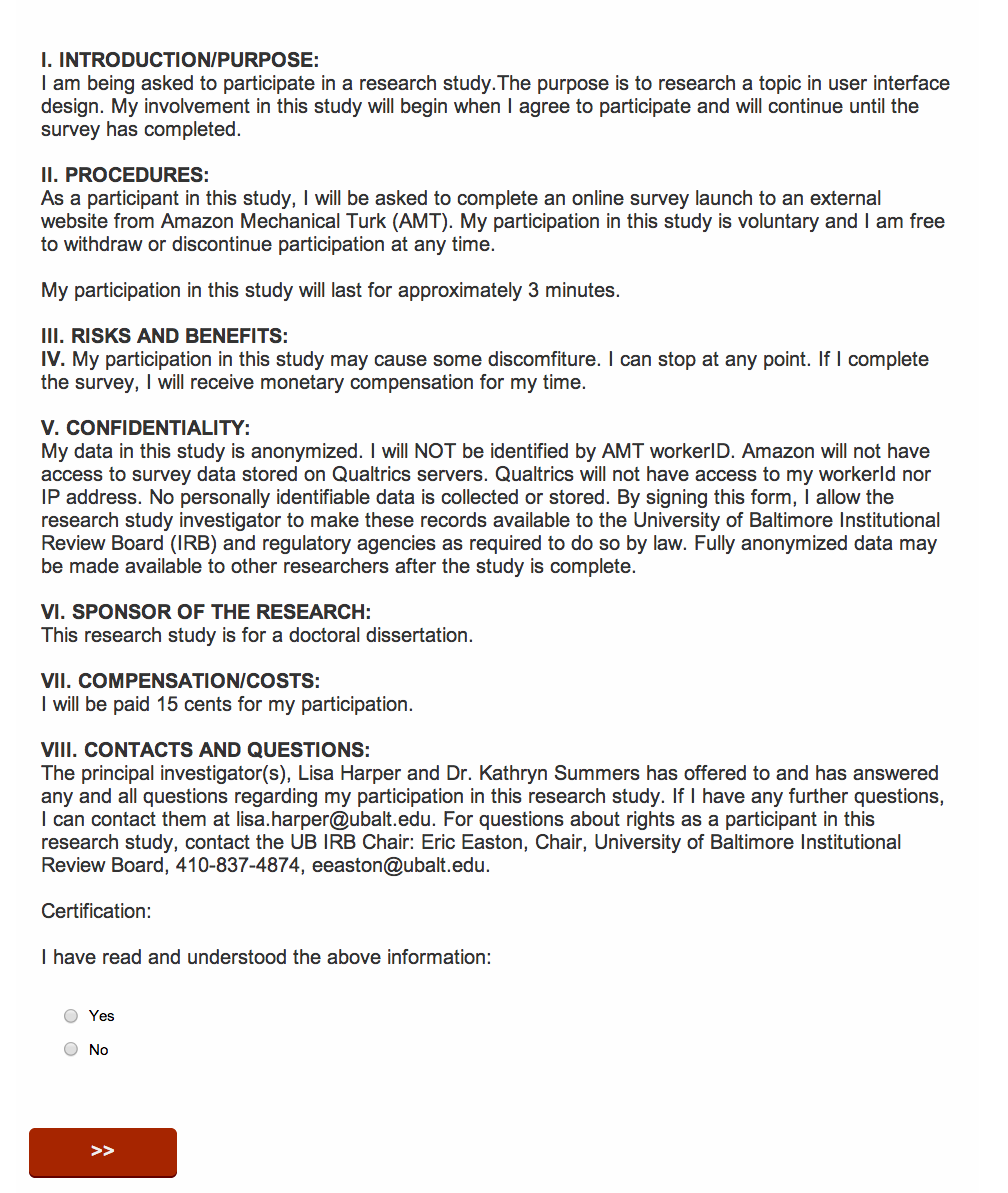
\includegraphics[scale=.40]{chapter4.tex/consent}
}
\end{figure}
%\setcounter{figure}{0} 
%
\chapter{AMT Terms of Service}
\label{amazon}
\begin{figure}[h!]
\centerline{
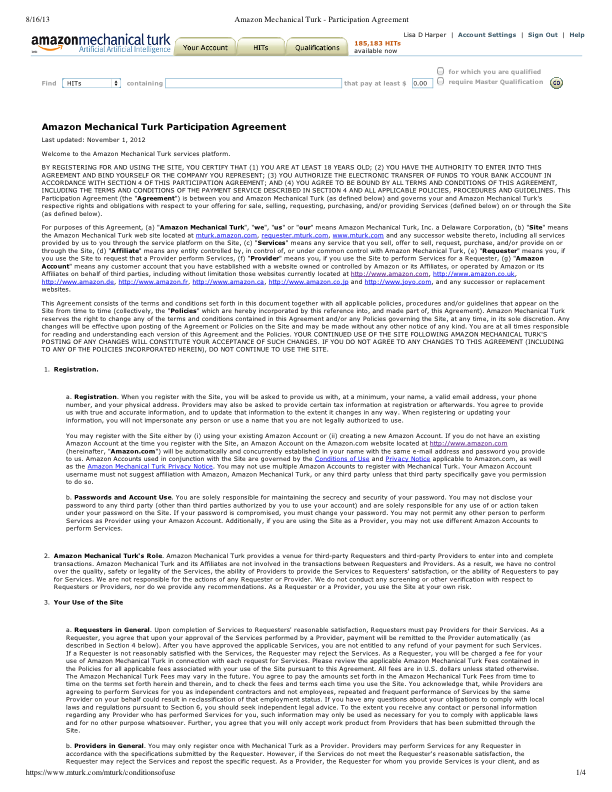
\includegraphics[scale=.6]{Appendices/amt-tos}
}
\end{figure}


%\setcounter{figure}{0} 
%
\chapter{Sample AMT Assignment Definition}
\label{assignment}
\lstset{numbers=none}
\begin{lstlisting}
title = Language study and demographic survey (3 min)
description: one task and then just a survey
keywords:survey, language

# how much you'll pay each subject
reward:.15

# how many subjects do you want
assignments:30

######################################
## HIT Timing Properties
######################################

# 60*10, 10 mins to finish a suvey
assignmentduration:600

# 60*60*24*2, 2 day to keep on mturk
hitlifetime:172800

# 10 seconds to auto approve the response
# 
autoapprovaldelay:10

######################################
## Qualification Properties
######################################

# user must have an approval rate of 90% or greater
qualification.1:000000000000000000L0
qualification.comparator.1:greaterthan
qualification.value.1:90
qualification.private.1:false

# user must be in the United States
qualification.2:00000000000000000071
qualification.comparator.2:equalto
qualification.locale.2:US
qualification.private.2:true
\end{lstlisting}


%\setcounter{figure}{0} 
%%**************************************************************
% Appendix
%*******************************************************
% If problems with the headers: get headings in appendix etc. right
%\markboth{\spacedlowsmallcaps{Appendix}}{\spacedlowsmallcaps{Appendix}}
\chapter{Survey Response}
\label{survey-response}
%%% LyX 2.0.6 created this file.  For more info, see http://www.lyx.org/.
%% Do not edit unless you really know what you are doing.
%\documentclass[english]{article}
%\usepackage[T1]{fontenc}
%\usepackage[latin9]{inputenc}
%\usepackage{longtable}
%\makeatletter

%%%%%%%%%%%%%%%%%%%%%%%%%%%%%% LyX specific LaTeX commands.
%% Because html converters don't know tabularnewline
%\providecommand{\tabularnewline}{\\}

%\makeatother

%\usepackage{babel}
%\begin{document}

%\setlength\LTleft{-30pt}            % default: \fill
%\setlength\LTright{-30pt}           % default: \fill
\footnotesize
\begin{longtable}{p{4cm} p{4cm}}
%\caption{Demographics (All Studies Combined)} \\
\textbf{Category} & \textbf{Percentage}\tabularnewline
\hline 
\hline 
\textbf{Age} & \tabularnewline
\hline 
18-24 & 28\%\tabularnewline
25-34 & 45\%\tabularnewline
35-49 & 20\%\tabularnewline
50-64 & 7\%\tabularnewline
64+ & 0\%\tabularnewline
\hline 
\textbf{Gender} & \tabularnewline
\hline 
Male & 53\%\tabularnewline
Female & 47\%\tabularnewline
\hline 
\textbf{Ethnic Identity} & \tabularnewline
\hline 
American Indian / Native American & 1\%\tabularnewline
Asian or Pacific Islander & 10\%\tabularnewline
Black / African American & 7\%\tabularnewline
Hispanic or Latin American & 7\%\tabularnewline
White / Caucasian & 73\%\tabularnewline
Near Eastern or Arabic & 0\%\tabularnewline
Other & 2\%\tabularnewline
\hline 
\textbf{Native Language} & \tabularnewline
\hline 
English & 97\%\tabularnewline
Other & 3\%\tabularnewline
\hline 
\textbf{English} & \tabularnewline
\hline 
A little English & 0\%\tabularnewline
Some English & 0\%\tabularnewline
Fluent English & 60\%\tabularnewline
Near-native English & 40\%\tabularnewline
\hline 
\textbf{Education} & \tabularnewline
\hline 
Some High School & 1\%\tabularnewline
High School Graduate & 13\%\tabularnewline
Some College / Associate Degree & 40\%\tabularnewline
College Degree & 37\%\tabularnewline
Post-graduate Degree & 9\%\tabularnewline
\hline 
\textbf{Income} & \tabularnewline
\hline 
Under 20,000 & 34\%\tabularnewline
20,000 - 30,000 & 19\%\tabularnewline
30,000 - 40,000 & 15\%\tabularnewline
40,000 - 50,000 & 10\%\tabularnewline
50,000+ & 22\%\tabularnewline
\hline 
\textbf{IT Job} & \tabularnewline
\hline
Yes & 20\%\tabularnewline
No & 80\%\tabularnewline
\hline 
\textbf{Internet Usage} & \tabularnewline
\hline 
Fewer than 4 hours per week & 2\%\tabularnewline
4-10 hours per week & 11\%\tabularnewline
10-25 hours per week & 30\%\tabularnewline
25+ hours per week & 57\%\tabularnewline
\hline 
\textbf{Shop Online} & \tabularnewline
\hline 
Never & 1\%\tabularnewline
Rarely & 17\%\tabularnewline
Sometimes & 30\%\tabularnewline
Often & 52\%\tabularnewline
\hline 
\textbf{Sense of Privacy in Public} & \tabularnewline
\hline 
Not private & 29\%\tabularnewline
A Little private & 30\%\tabularnewline
Somewhat private & 29\%\tabularnewline
Private & 9\%\tabularnewline
Very private & 3\%\tabularnewline
\hline 
\textbf{Sense of Privacy at Home} & \tabularnewline
\hline 
Not private & 4\%\tabularnewline
A Little private & 10\%\tabularnewline
Somewhat private & 23\%\tabularnewline
Private & 37\%\tabularnewline
Very private & 26\%\tabularnewline
\hline 
\textbf{Importance of Online Privacy } & \tabularnewline
\hline 
Not much of an issue & 7\%\tabularnewline
Somewhat important & 51\%\tabularnewline
Really important & 42\%\tabularnewline
\hline 
\textbf{Steps to Protect Privacy} & \tabularnewline
\hline 
Don't know how to protect & 8\%\tabularnewline
Know how but not consistent & 49\%\tabularnewline
Know how and take measures & 43\%\tabularnewline
\hline 
\textbf{Know what a tracking cookie is} & \tabularnewline
\hline 
Yes & 91\%\tabularnewline
No & 9\%\tabularnewline
\hline 
\textbf{DNT means...} & \tabularnewline
\hline 
Do not show targeted advertising & 20\%\tabularnewline
Do not track across sites & 54\%\tabularnewline
Do not track on this site & 47\%\tabularnewline
Do not collect information & 48\%\tabularnewline
Do not store information & 43\%\tabularnewline
\hline 
\textbf{Would Turn off Tracking if Easy?} & \tabularnewline
\hline 
Yes & 91\%\tabularnewline
No & 9\%\tabularnewline
\hline 
\textbf{Browser Configured Opt-Out} & \tabularnewline
\hline 
Yes & 55\%\tabularnewline
No & 45\%\tabularnewline
\hline 
\textbf{Use a Browser Plugin for Privacy Protection} & \tabularnewline
\hline 
Yes & 73\%\tabularnewline
No & 27\%\tabularnewline
\hline 
\textbf{Total} & \textbf{1158}\tabularnewline
\hline 
\end{longtable}
%\end{document}

%% LyX 2.0.6 created this file.  For more info, see http://www.lyx.org/.
%% Do not edit unless you really know what you are doing.
%\documentclass[english]{article}
%\usepackage[T1]{fontenc}
%\usepackage[latin9]{inputenc}

%\makeatletter

%%%%%%%%%%%%%%%%%%%%%%%%%%%%%% LyX specific LaTeX commands.
%% Because html converters don't know tabularnewline
%\providecommand{\tabularnewline}{\\}

%\makeatother

%\usepackage{babel}
%\begin{document}

\begin{longtable}{p{4cm} p{4cm} p{3cm}}
\caption{Aggregate Demographic Profile and Survey Response} \\
\textbf{Category} & \textbf{Experiment 3} & \textbf{Total}\tabularnewline
\hline 
\hline 
\textbf{Age} &  & \tabularnewline
\hline 
18-24 & 29\% & 28\%\tabularnewline
25-34 & 44\% & 45\%\tabularnewline
35-49 & 17\% & 20\%\tabularnewline
50-64 & 10\% & 7\%\tabularnewline
64+ & 0\% & 0\%\tabularnewline
\hline 
\textbf{Gender} &  & \tabularnewline
\hline 
Male & 63\% & 53\%\tabularnewline
Female & 37\% & 47\%\tabularnewline
\hline 
\textbf{Ethnic Identity} &  & \tabularnewline
\hline 
American Indian / Native American & 0\% & 1\%\tabularnewline
Asian or Pacific Islander & 10\% & 10\%\tabularnewline
Black / African American & 3\% & 7\%\tabularnewline
Hispanic or Latin American & 5\% & 7\%\tabularnewline
White / Caucasian & 82\% & 73\%\tabularnewline
Near Eastern or Arabic & 0\% & 0\%\tabularnewline
Other & 2\% & 2\%\tabularnewline
\hline 
\textbf{Native Language} &  & \tabularnewline
\hline 
English & 99\% & 97\%\tabularnewline
Other & 1\% & 3\%\tabularnewline
\hline 
\textbf{English} &  & \tabularnewline
\hline 
A little English & 0\% & 0\%\tabularnewline
Some English & 0\% & 0\%\tabularnewline
Fluent English & 0\% & 60\%\tabularnewline
Near-native English & 100\% & 40\%\tabularnewline
\hline 
\textbf{Education} &  & \tabularnewline
\hline 
Some High School & 1\% & 1\%\tabularnewline
High School Graduate & 17\% & 13\%\tabularnewline
Some College or Associate Degree & 39\% & 40\%\tabularnewline
College Degree & 35\% & 37\%\tabularnewline
Post-graduate Degree & 8\% & 9\%\tabularnewline
\hline 
\textbf{Income} &  & \tabularnewline
\hline 
Under 20,000 & 30\% & 34\%\tabularnewline
20,000 - 30,000 & 25\% & 19\%\tabularnewline
30,000 - 40,000 & 13\% & 15\%\tabularnewline
40,000 - 50,000 & 13\% & 10\%\tabularnewline
50,000+ & 20\% & 22\%\tabularnewline
\hline 
\textbf{IT Job} &  & \tabularnewline
\hline
Yes & 21\% & 20\%\tabularnewline
No & 79\% & 80\%\tabularnewline
\hline 
\textbf{Internet Usage} &  & \tabularnewline
\hline 
Fewer than 4 hours per week & 1\% & 2\%\tabularnewline
4-10 hours per week & 13\% & 11\%\tabularnewline
10-25 hours per week & 41\% & 30\%\tabularnewline
25+ hours per week & 45\% & 57\%\tabularnewline
\hline 
\textbf{Shop Online} &  & \tabularnewline
\hline 
Never & 1\% & 1\%\tabularnewline
Rarely & 20\% & 17\%\tabularnewline
Sometimes & 59\% & 30\%\tabularnewline
Often & 21\% & 52\%\tabularnewline
\hline 
\textbf{Sense of Privacy in Public} &  & \tabularnewline
\hline 
Not private & 31\% & 29\%\tabularnewline
A Little private & 34\% & 30\%\tabularnewline
Somewhat private & 23\% & 29\%\tabularnewline
Private & 11\% & 9\%\tabularnewline
Very prvate & 1\% & 3\%\tabularnewline
\hline 
\textbf{Sense of Privacy at Home} &  & \tabularnewline
\hline 
Not private & 5\% & 4\%\tabularnewline
A Little private & 15\% & 10\%\tabularnewline
Somewhat private & 23\% & 23\%\tabularnewline
Private & 34\% & 37\%\tabularnewline
Very prvate & 24\% & 26\%\tabularnewline
\hline 
\textbf{Importance of Online Privacy } &  & \tabularnewline
\hline 
Not much of an issue & 8\% & 7\%\tabularnewline
Somewhat important & 50\% & 51\%\tabularnewline
Really important & 42\% & 42\%\tabularnewline
\hline 
\textbf{Steps to Protect Privacy} &  & \tabularnewline
\hline 
Don't know how to protect & 12\% & 8\%\tabularnewline
Know how but not consistent & 38\% & 49\%\tabularnewline
Know how and take measures & 50\% & 43\%\tabularnewline
\hline 
\textbf{Know what a tracking cookie is} &  & \tabularnewline
\hline 
Yes & 90\% & 91\%\tabularnewline
No & 10\% & 9\%\tabularnewline
\hline 
\textbf{DNT means...} &  & \tabularnewline
\hline 
Do not show targeted advertising & 17\% & 20\%\tabularnewline
Do not trakc across sites & 44\% & 54\%\tabularnewline
Do not track on this site & 49\% & 47\%\tabularnewline
Do not collect information & 39\% & 48\%\tabularnewline
Do not store information & 38\% & 43\%\tabularnewline
\hline 
\textbf{Would Turn off Tracking if Easy?} &  & \tabularnewline
\hline 
Yes & 88\% & 91\%\tabularnewline
No & 12\% & 9\%\tabularnewline
\hline 
\textbf{Browser Configured Opt-Out} &  & \tabularnewline
\hline 
Yes & 54\% & 55\%\tabularnewline
No & 46\% & 45\%\tabularnewline
\hline 
\textbf{Use a Browser Plugin for Privacy Protection} &  & \tabularnewline
\hline 
Yes & 70\% & 73\%\tabularnewline
No & 30\% & 27\%\tabularnewline
\hline 
\textbf{Total} & \textbf{100} & \textbf{1158}\tabularnewline
\end{longtable}
%\end{document}

%\setcounter{figure}{0} 
%
\chapter{Experiment 1 Conditions}
\label{exp1-conditions}
\begin{figure}[h!]
\centerline{
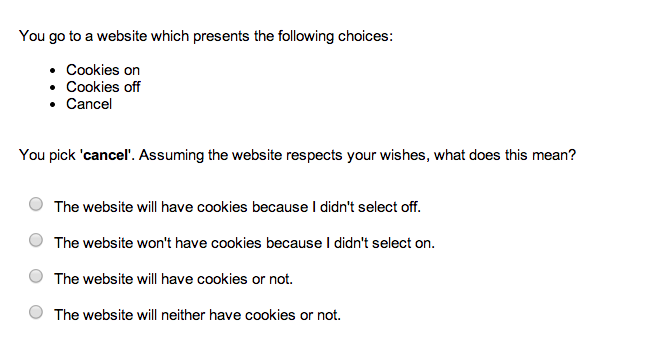
\includegraphics[scale=.5]{chapter5.tex/textnocpcookie}
}
\caption{Text, No Deontic Force, Cookie Condition}
\end{figure}


\begin{figure}[h!]
\centerline{
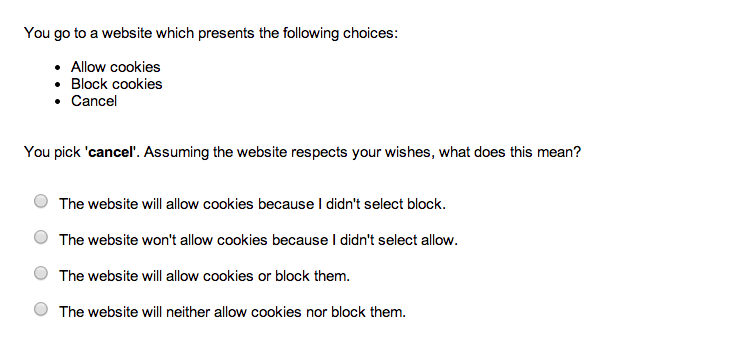
\includegraphics[scale=.5]{chapter5.tex/textcpcookie}
}
\caption{Text, Deontic Force, Cookie Condition}
\end{figure}


\begin{figure}[h!]
\centerline{
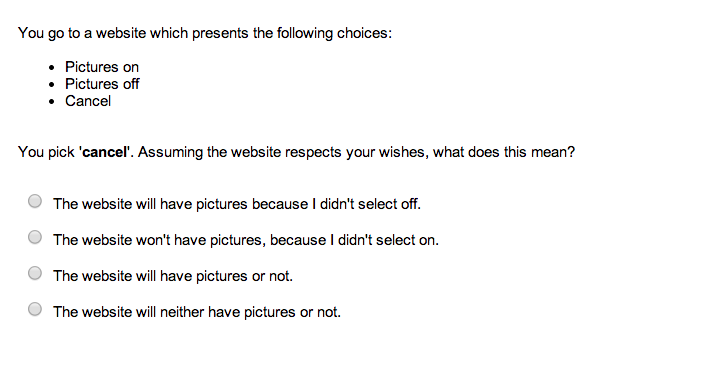
\includegraphics[scale=.5]{chapter5.tex/textnocppic}
}
\caption{Text, No Deontic Force, Picture Condition}
\end{figure}


\begin{figure}[h!]
\centerline{
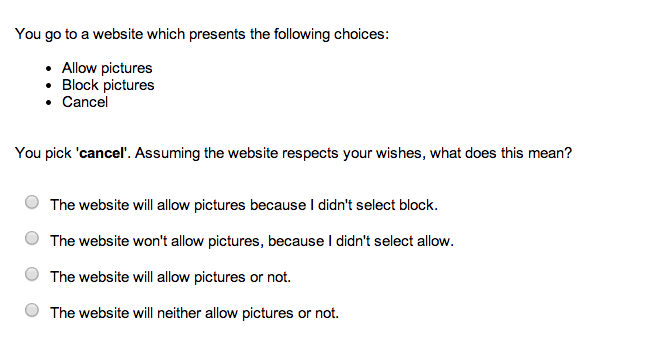
\includegraphics[scale=.5]{chapter5.tex/textcppic}
}
\caption{Text, Deontic Force, Picture Condition}
\end{figure}


\begin{figure}[h!]
\centerline{
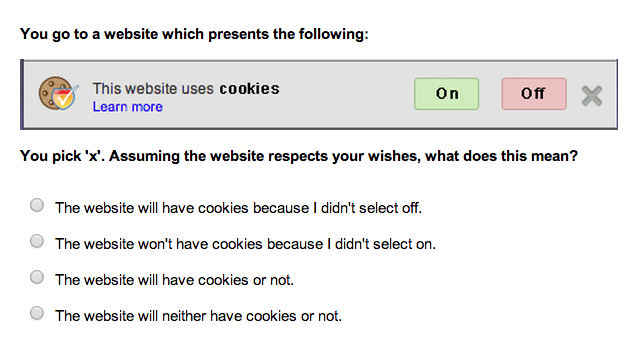
\includegraphics[scale=.5]{chapter5.tex/dialognocpcookie}
}
\caption{Mixed-Modal, No Deontic Force, Cookie Condition}
\end{figure}


\begin{figure}[h!]
\centerline{
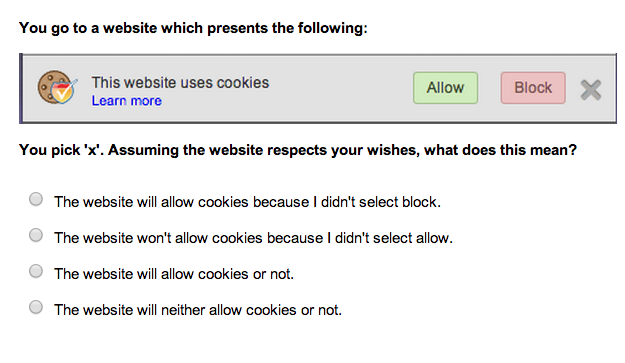
\includegraphics[scale=.5]{chapter5.tex/dialogcpcookie}
}
\caption{Mixed-Modal, Deontic Force, Cookie Condition}
\end{figure}



\begin{figure}[h!]
\centerline{
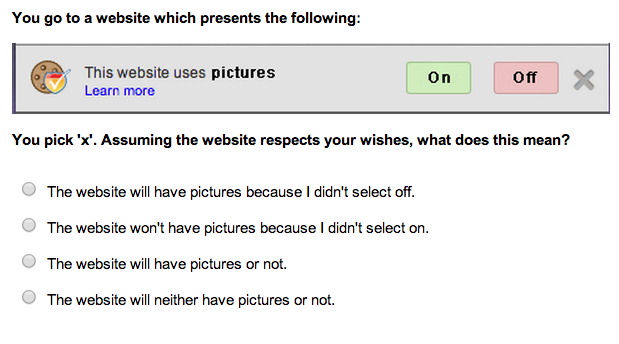
\includegraphics[scale=.5]{chapter5.tex/dialognocppic}
}
\caption{Mixed-Modal, No Deontic Force, Picture Condition}
\end{figure}


\begin{figure}[h!]
\centerline{
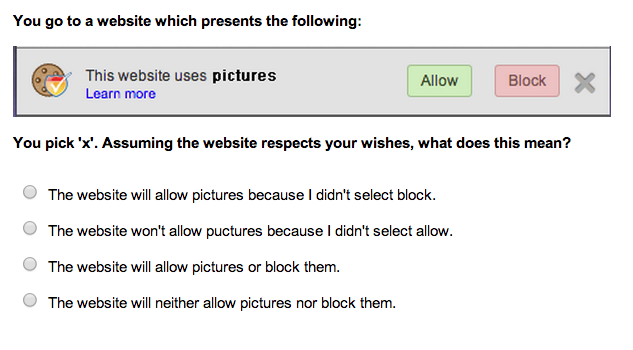
\includegraphics[scale=.5]{chapter5.tex/dialogcppic}
}
\caption{Mixed-Modal, Deontic Force, Picture Condition}
\end{figure}
%\setcounter{figure}{0} 
%
\chapter{Experiment 1 Raw Results}
\label{exp1-raw}
\begin{figure}[h!]
\centerline{
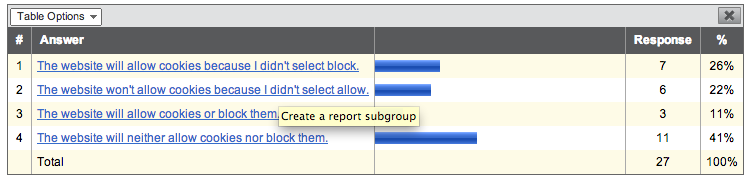
\includegraphics[scale=.44]{chapter5.tex/raw1}
}
\caption{Text, Deontic Force, Cookie Condition}
\end{figure}


\begin{figure}[h!]
\centerline{
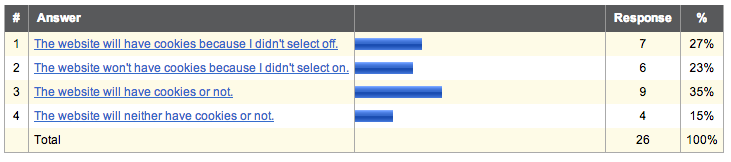
\includegraphics[scale=.45]{chapter5.tex/raw2}
}
\caption{Text, No Deontic Force, Cookie Condition}
\end{figure}


\begin{figure}[h!]
\centerline{
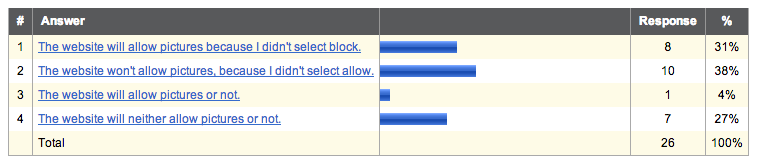
\includegraphics[scale=.45]{chapter5.tex/raw3}
}
\caption{Text, Deontic Force, Picture Condition}
\end{figure}


\begin{figure}[h!]
\centerline{
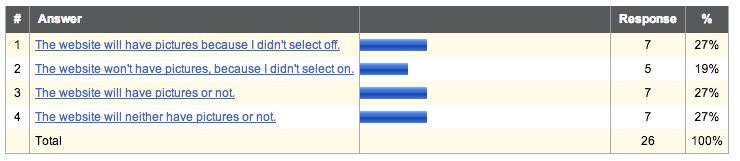
\includegraphics[scale=.45]{chapter5.tex/raw4}
}
\caption{Text, No Deontic Force, Picture Condition}
\end{figure}


\begin{figure}[h!]
\centerline{
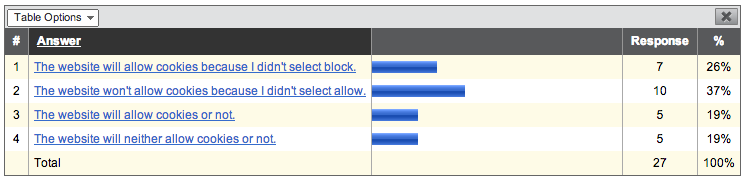
\includegraphics[scale=.44]{chapter5.tex/raw5}
}
\caption{Graphic, Deontic Force, Cookie Condition}
\end{figure}


\begin{figure}[h!]
\centerline{
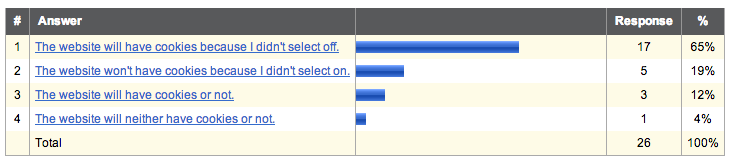
\includegraphics[scale=.45]{chapter5.tex/raw6}
}
\caption{Graphic, No Deontic Force, Cookie Condition}
\end{figure}


\begin{figure}[h!]
\centerline{
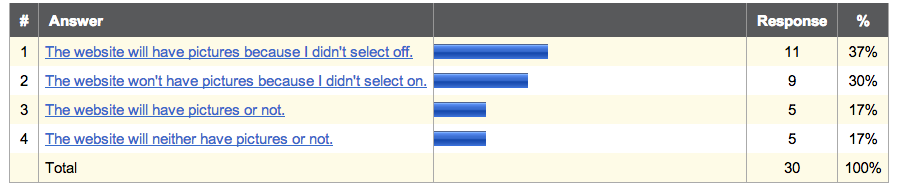
\includegraphics[scale=.38]{chapter5.tex/raw7}
}
\caption{Graphic, No Deontic Force, Picture Condition}
\end{figure}


\begin{figure}[h!]
\centerline{
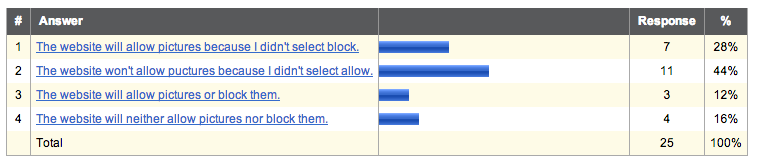
\includegraphics[scale=.45]{chapter5.tex/raw8}
}
\caption{Graphic, Deontic Force, Picture Condition}
\end{figure}
%\setcounter{figure}{0} 
%
\chapter{Participant Survey}
\label{survey}
%\begin{parbox}{\textwidth}
%\centering
%\begin{figure}
%\begin{sideways}
%\centerline{
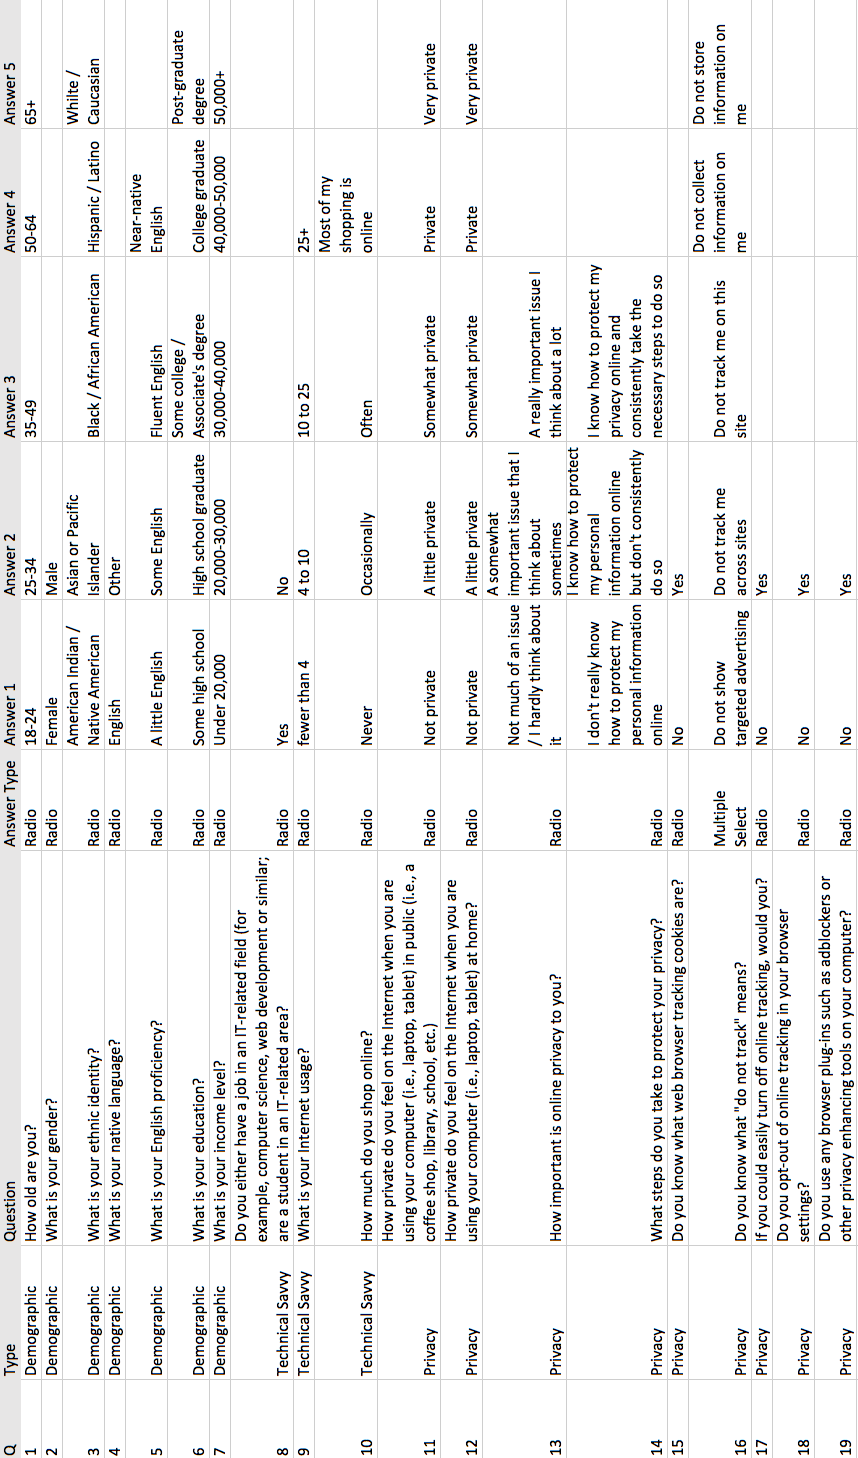
\includegraphics[scale=.38]{Appendices/survey-rotated}
%}
%\end{sideways}
%\end{figure}
%\end{parbox}

 %

%----------------------------------------------------------------------------------------
%	POST-CONTENT THESIS PAGES
%----------------------------------------------------------------------------------------

\cleardoublepage% Bibliography

\label{app:bibliography} % Reference the bibliography elsewhere with \autoref{app:bibliography}

\manualmark
\markboth{\spacedlowsmallcaps{\bibname}}{\spacedlowsmallcaps{\bibname}} 
\refstepcounter{dummy}

\addtocontents{toc}{\protect\vspace{\beforebibskip}} % Place the bibliography slightly below the rest of the document content in the table of contents
\addcontentsline{toc}{chapter}{\tocEntry{\bibname}}

%\bibliographystyle{plainnat}
%\bibliographystyle{apalike2}
\bibliographystyle{apacite}

%\bibliography{Bibliography}
\bibliography{bib} % Bibliography

\end{document}